% Standalone figure for the Statistical Mechanics notes.
% Build: pdflatex unary-PT.tex  (or run build.sh in this folder)
\documentclass[11pt,tikz,border=2pt]{standalone}
\usepackage{amsmath,amssymb}
\usetikzlibrary{arrows.meta, positioning}
\begin{document}
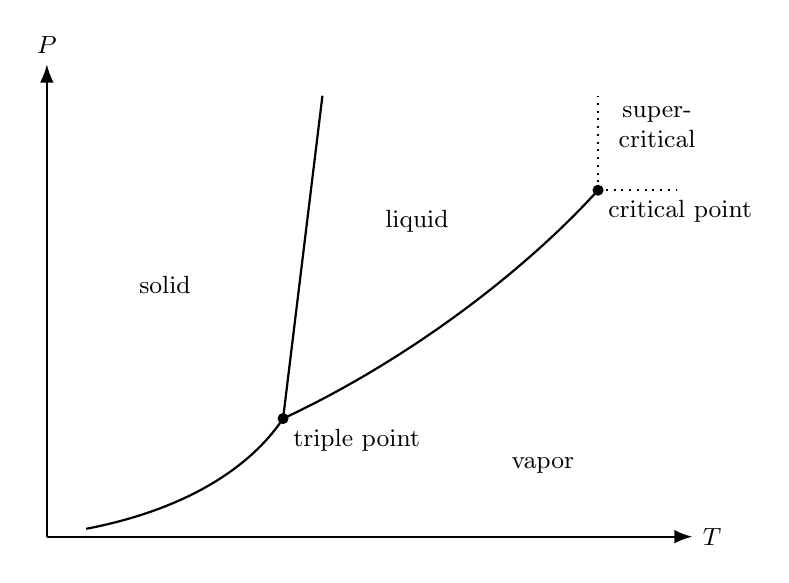
\begin{tikzpicture}[font=\small, >=Latex, line width=0.8pt]
    % axes
    \draw[->] (0,0) -- (8.2,0) node[right] {$T$};
    \draw[->] (0,0) -- (0,6) node[above] {$P$};
    % solid--vapor (sublimation) curve
    \draw (0.5,0.1) .. controls (1.8,0.35) and (2.6,0.9) .. (3,1.5);
    % liquid--vapor (vaporization) curve, ending at the critical point
    \draw (3,1.5) .. controls (4.5,2.2) and (6,3.3) .. (7,4.4);
    % solid--liquid (melting) curve
    \draw (3,1.5) -- (3.5,5.6);
    % triple and critical points
    \fill (3,1.5) circle (2pt);
    \fill (7,4.4) circle (2pt);
    \node[below right] at (3,1.5) {triple point};
    \node[below right] at (7,4.4) {critical point};
    % supercritical boundaries (no transition)
    \draw[dotted] (7,4.4) -- (7,5.6);
    \draw[dotted] (7,4.4) -- (8,4.4);
    % phase labels
    \node at (1.5,3.2) {solid};
    \node at (4.7,4.0) {liquid};
    \node at (6.3,0.9) {vapor};
    \node[align=center] at (7.75,5.2) {super-\\critical};
\end{tikzpicture}
\end{document}
